% !TEX root = ../my-thesis.tex
%
\chapter{AutoML via an Ensemble of Optimizers}
\label{sec:approach}
As outlined in the previous chapter, in theory any optimization approach under a budget is limited to a set of problem classes, where it can find a solution that is better than any solution another optimization approach could find for the same problem class, i.e. where the approach is superior.
For an actual use-case, as for instance AutoML, it would be necessary to either have significant domain knowledge or to had conducted a broad empirical evaluation to select the optimizer that have a high chance of performing superior for a newly encountered problem class.
This can be avoided, if during the optimization process a set of optimizers would be evaluated in the context of the presented optimization problem and the most apt one would be applied automatically.\newline
Furthermore, it was argued, how a separation of the optimization space into model selection and model configuration spaces by optimization space transformations could be beneficial.
The anticipated advantages are a speed-up at first, because the dimensionality of the input space for an optimizer can be reduced.
Secondly, the best suited optimizer for the optimization space of the model configuration of a constructed pipeline can be selected independently for each different result of the model selection steps.

Although this approach could be generalized to any form of algorithm selection and hyperparameter configuration problem, this thesis focusses on the AutoML use-case and therewith has to address well suited machine learning pipelines as an expected output for a wide variety of datasets as an input.
Thus, the constructed pipelines should be able to be as sophisticated as necessary to suit the complexity of any possible input dataset.
Therewith, the approach has the additional requirement of preventing overly stringent limitations of the pipeline topology such as a fix length or solely linear compositions.\newline
In the following chapter such a method is presented and applied to the AutoML use-case.
This approach is explained in the following steps in separate sections:
\begin{enumerate}
    \item A short overview how model selection and configuration spaces can be separated for this approach
    \item The structure of the model selection optimization space, with a focus on how the optimization in this space is performed to enable the selection of different optimizers for model configuration out of an embedded optimizer ensemble
    \item The structure of the model configuration optimization space and which benefits can be utilized from using and re-using the different optimizers of the ensemble
\end{enumerate}

\section{Separation of Model Selection and Configuration}
\label{sec:approach:separation}
A usual AutoML optimization search space is a joint space for model selection and model configuration consisting of a set of components, which can be used to construct a machine learning pipeline, and based on the selected components, a valid configuration has to be created.
Since in the joint optimization space the selected components are not known beforehand, the dimensionality of this space has to be selected for a fix parametrization size.
Hence, the model configuration can only create parameter configurations with a pre-defined size as a constraint and the set of pipeline components for model selection can only contain components whose configuration does not exceed this size.\newline
If the model selection and the model configuration steps are performed sequentially on separated optimization spaces, the dimensionality of the model configuration space can depend on the outcome of the model selection step and have the necessary dimensionality for the constructed pipelines parametrization.\newline
Similar to ReinBo and Mosaic, the model selection space of this approach is represented by a tree structure.
After the optimization method reaches a leaf node and has therewith a complete and valid pipeline structure, the size of the required configuration becomes clear.
Any leaf node is for this reason the connection point and foundation for a model configuration space and the configuration requirements can be deduced.
Thus, dimensionality and structure of the optimization space for the model configuration can be determined from the configuration requirements of the pipeline represented in this leaf node.

\section{Model Selection with MCTS}
\label{sec:approach:selection}
While the overall goal of the model selection step is to construct a pipeline out of a set of pipeline components, in this approach two additional sub-goals come as supplementary requirements:
\begin{enumerate}
    \item The constructed pipeline should be able to be constructed more flexible and more sophisticated than in ReinBo and Mosaic, i.e. have an unrestricted length and no constraints regarding the topology.
    \item The model selection step should be able to evaluate the different optimization methods and their performance regarding the input dataset or even regarding the model configuration for specific pipeline components in the context of the dataset.
    With such an approach, the most suitable optimizer can be detected and exploited, which will be the key concept in this approach for creating an optimizer ensemble.
\end{enumerate}
In the following, both sub-goals are addressed.
The next two sub-sections tackle the first sub-goal by modelling the model selection process as a graph search problem at first and describing this search graph in more detail afterwards.
Thereafter, in the third sub-section a formalization of the ensemble concept for multiple optimizers is given in the form of a Multi-Armed Bandit problem.
Finally, in the fourth sub-section it is illustrated how both sub-goals can be achieved during the model selection by performing an MCTS.

\subsection{Model Selection as a Graph Search Problem}
\label{sec:approach:selection:search}
A machine learning pipeline can vary significantly in structure and complexity.
For example, using a decision tree as the only component is a valid pipeline as well as many components in a more sophisticated topology such as the pipeline in Fig. ~\ref{fig:approach:complex-pipeline}.
Depending on the concrete input dataset, both levels of pipeline complexity could be the optimal output of the model selection step.
\begin{figure}[ht!]
    \centering
    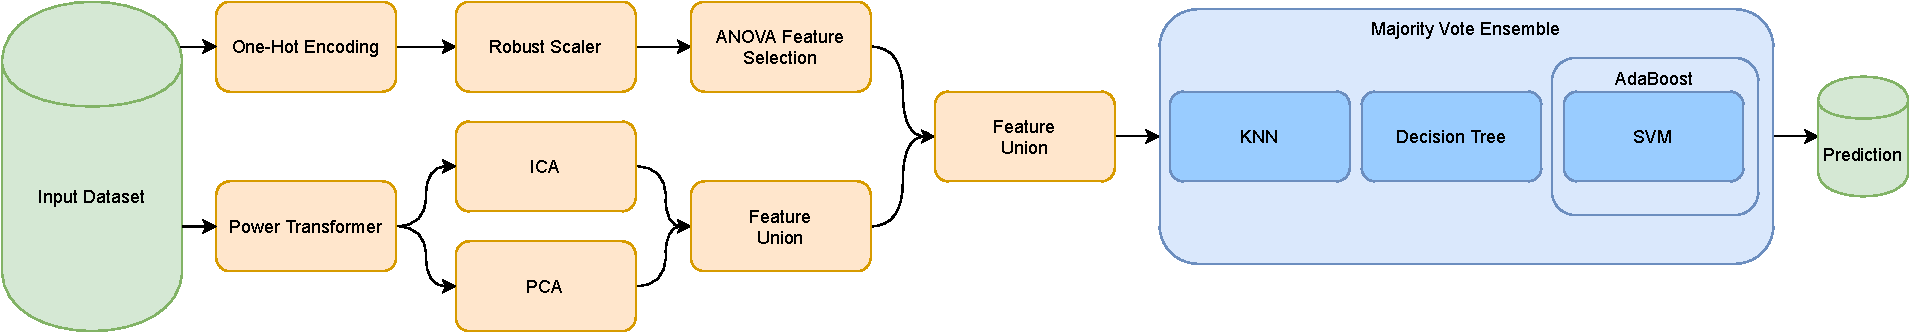
\includegraphics[width=\textwidth]{gfx/Figures/Approach/ComplexPipeline.pdf}
    \caption[An example of a complex machine learning pipeline with an increased length and a non-linear topology.]{An example of a complex machine learning pipeline with a higher length and a non-linear topology. Input dataset and output prediction data are shown in green, pre-processing components in orange and the machine learning components constructing the machine learning algorithm in blue.}
    \label{fig:approach:complex-pipeline}
\end{figure}

In their current implementation, ReinBo and Mosaic solve their model selection tasks by defining a fix pipeline length and creating a model selection tree containing the combinatorial possible combination with this length and the given component set. 
Although it would be possible to increase the maximal pipeline length of the two approaches with minor modifications, the concept, where each layer represents one respective open component slot of the result pipeline, does not allow more complex pipeline topologies than linear.\newline
Other approaches, as for example ML-Plan, TPOT or RECIPE utilize respectively hierarchical task network planning (\textit{HTN planning}) combined with a best-first search, or expression trees and formal grammars together with genetic programming, to achieve a more unconstrained model selection optimization space.
The optimizer ensembles of this approach try to achieve two aspects.
First, the optimizers of the ensemble should to share the gathered knowledge between each other and utilize it.
Second, during the ongoing AutoML workflow, the best optimizer for the given problem instance should be identified and exploited.
This second aspect will be controlled by the model selection. 
For this control function, an MCTS is a suitable choice (this is reasoned in~\ref{sec:approach:selection:mcts}), which is a heuristic graph search algorithm like the best-first search as in ML-Plan.
The search of this ensemble approach will take this HTN planning approach as a foundation to construct the model selection space in the form of a tree.

As the name suggests, HTN planning is based around the notion of tasks and usually one task is given as the planning problem input.
The goal of the planning algorithms is now to construct a plan to solve this input task.
In the case of HTN planning, tasks can either be primitive tasks or compound task.\newline
Primitive tasks are simple enough to be directly achievable without the need for further planning or other calculations.
Compound tasks on the other hand, are not directly realizable and it is necessary to further decompose the task.
Usually, the input task is a compound task, because otherwise there would be no need for any planing.
This planning is done for HTN planning in the form of decompositions of compound tasks.\newline
Each compound task can be decomposed into one or most commonly two or more sub-tasks.
Such sub-tasks of a compound task can be primitive tasks, compound tasks, or a mixture of both.
If a compound task can be decomposed into solely primitive tasks, this task is directly solvable via the actions of the primitive tasks.
But if the decomposition of the compound task consists of at least one compound tasks, this child compound task needs to be decomposed recursively as well until it becomes solvable and this solution can be used to solve the original compound task.
Depending on the planning domain, there are decomposition rules where a compound task has one or more possible decompositions.\newline
For example in an AutoML setting, one compound tasks could be something like a formalized form of "\textit{Construct a machine learning pipeline out of a set of components}".
In the same context, an example for a primitive task could be "\textit{Use a decision tree as a learning algorithm for the pipeline}" as this task can be directly transformed into a pipeline construction command.
The exemplaric AutoML compound task "\textit{Construct a machine learning pipeline out of a set of components}" could be decomposed for example into the to smaller compound tasks "\textit{Construct a pre-processing pipeline out of a set of pre-processing components}" and "\textit{Construct a learning algorithm out of a set of machine learning components}".

With this decomposition of compound tasks into different sub-tasks, the hierarchical aspect of HTN planning is added.
A plan as the solution of the planning problem is therefore a task-tree, where each leaf node is a primitive task and each inner node is a compound task.
To create a search tree for an HTN planning problem, solution states, i.e. solved or incomplete task-trees, as well as planning operations to solve an incomplete task-tree, i.e. selecting and applying decomposition rules, need to be represented with nodes and edges.
Solved or incomplete tasks-trees are also called plans or plan prefixes in the incomplete case.\newline
Here is one common possibility to have each node represent a task-tree and each outgoing edge is a decomposition rule that is applicable to the task-tree of the node.
This edges are therefore connected to nodes, where the represented task-tree is the result of applying this decomposition rule on the previous task-tree.
For a bigger HTN problem an unsolved task-tree will contain a high number of undecomposed compound nodes and therefore an immense amount of decomposition rules would be applicable.
To reduce the maximum degree of the graph and therefore the memory and runtime complexity of most search algorithms, there should not be an outgoing edge for the applicable decomposition rules of each undecomposed compound task.
A simplification is to create an ordering for the undecomposed compound task of the nodes task tree and only create outgoing edges for decomposition rules, which are applicable to the first compound task of this ordering.
The representation of one simple incomplete task tree and two applicable decomposition rules for the first compound task of an ordering is illustrated in Fig.~\ref{fig:approach:htn-planning}.
\begin{figure}[ht!]
    \centering
    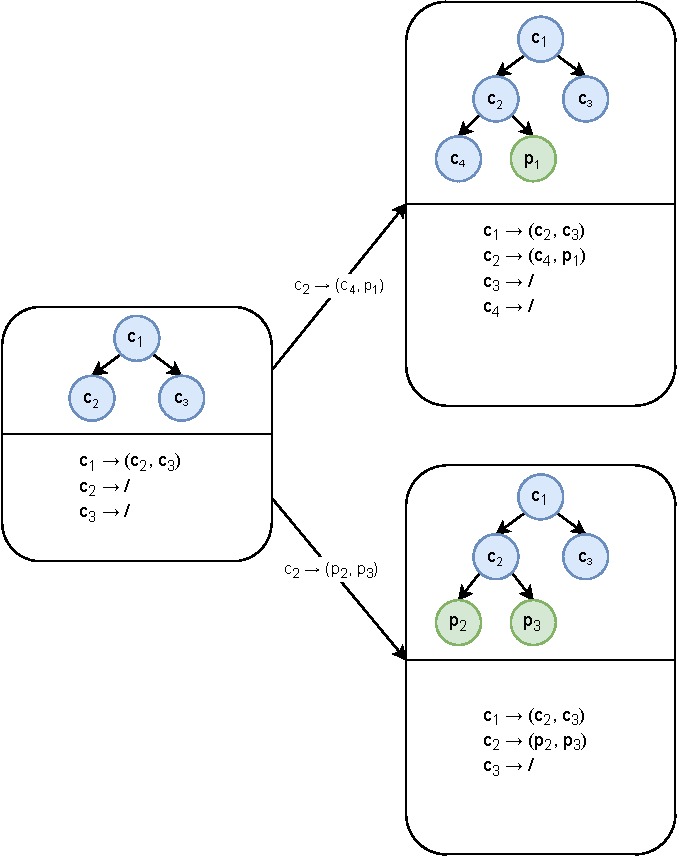
\includegraphics[height=0.5\textheight]{gfx/Figures/Approach/HTN.pdf}
    \caption[An example of a partial HTN planning search tree for a simple planning problem.]{An example of a partial HTN planning search tree for a simple planning problem. Each node is illustrated with the task-tree for the partially solved plan up to this point in its upper half, where compound task nodes are blue and primitive task nodes are green.
    In the lower half are all involved compound tasks listed in the utilized ordering.
    If any decomposition rule was already applied for a compound task, it is listed here as well.
    The first node on the left has already utilized a decomposition for compound task $c_1$ into $c_2$ and $c_3$.
    In this ordering the first undecomposed compound task is $c_2$ and since two decomposition rules $c_2 \rightarrow (c_4, p_1)$ and $c_2 \rightarrow (p_2, p_3)$ are applicable, the node of this task-tree has two outgoing edges to nodes, where the corresponding decomposition rule was applied to the represented task tree.
    After applying the second decomposition rule, $c_2$ has solely primitive tasks as sub-tasks and can therefore be marked as solved.
    In the case of the first decomposition rule, $c_4$ needs to be decomposed and solved before $c_2$ can would be solved.
    }
    \label{fig:approach:htn-planning}
\end{figure}

\subsection{Description of the Search Space Graph}
\label{sec:approach:selection:graph}
The examples of HTN tasks in~\ref{sec:approach:selection:search} are given as instructions in plain english but this cannot be used in an algorithm and therefore a formalization is necessary.
With a suitable formalization and corresponding data model, the HTN planning domain is adjustable and expandable for the exact use-case.
Based on this adjustments and expansions, it is possible to modify valid pipeline topologies and the set of pipeline components for pipeline construction for the AutoML use-case.\newline
While attempting pipeline constructions, it is not possible to create arbitrary pipeline graphs because components often expect one specific type of input that can only be provided from other components, which have this type as their output type.
Additionally, sometimes the selection of some components implies the requirement of selecting certain other components.
For example if an ensemble method was selected as a learning algorithm, the components that are used to be the predictors of the ensemble must be learning algorithm components and cannot be pre-processing components.

To incorporate such constraints into tasks and decomposition rules, ML-Plan utilizes a simple type system in the form of required and provided interfaces as an additional abstraction layer above the tasks .
Each task has one or more type definitions which represent certain properties of the solution to the associated task.
For example, the primitive task of using a decision tree as well as the compound task of creating an ensemble learning algorithm out of several other learning algorithms would both offer a solution in the form of a machine learning algorithm.
Both of them could have something like \texttt{Classifier} or \texttt{Learner} as their solution type and therewith as the types of interfaces they provide.\newline
On the other hand, compound tasks are only solvable if they get solutions of certain types as the results of the sub-tasks they are decomposed into.
For example, a Stacking classifier can only be based on other classifiers, i.e. solutions with types like \texttt{Classifier}.
Thus, each compound task has one or more required interfaces, which represent the necessary solution types of the tasks the compound task could be decomposed into.\newline
Decomposition rules are now simple matching rules, i.e. which required interfaces can be satisfied with which provided interface.
Of course, as the easiest form of matching rule it is possible that this interface types must be identical.
A compound task with a single required interface of type $a$ can only be decomposed into another task, which has $a$ as one of its provided interface types.
With such a definitions of required and provided interface types for each task, it is straightforward to incorporate construction constraints into the planning problem without the need to write an extensive list of decomposition rules.
These constraints can be pipeline topology specific constraints like splits into two sub-pipelines and uniting such sub-pipelines again, or machine learning specific constraints as for example creating ensembles out of classifiers.

The overall pipeline structure, for example Pre-Processing + Learning Algorithm or Pre-Processing + Learning Algorithm + Post-Processing, can be encoded in the decomposition rules for input tasks.
Every actual pipeline component, which shall be included in the pipeline construction of a solved task tree, will be represented as primitive tasks.\newline
Non-linear topologies like creating parallel pre-processing sub-pipelines can be for example achieved with a Feature Union pipeline component, which has one or more types of pre-processing components as required interfaces.
Pipelines with a dynamic length can be achieved in a similar manner to generating sequences with an unlimited length in a regular grammar, where a pipeline can either be decomposed into just a component or a component and a pipeline.\newline
A simple HTN planning space for a very small AutoML model selection space is illustrated in~\ref{fig:approach:htn-automl}.
For a better understanding, an example of a more detailed and sophisticated AutoML HTN planning space is given in Appendix~\ref{sec:appendix:htn-space}.
It is written in the JSON schema, which is defined in~\ref{sec:implementation:json}.
\begin{figure}[ht!]
    \centering
    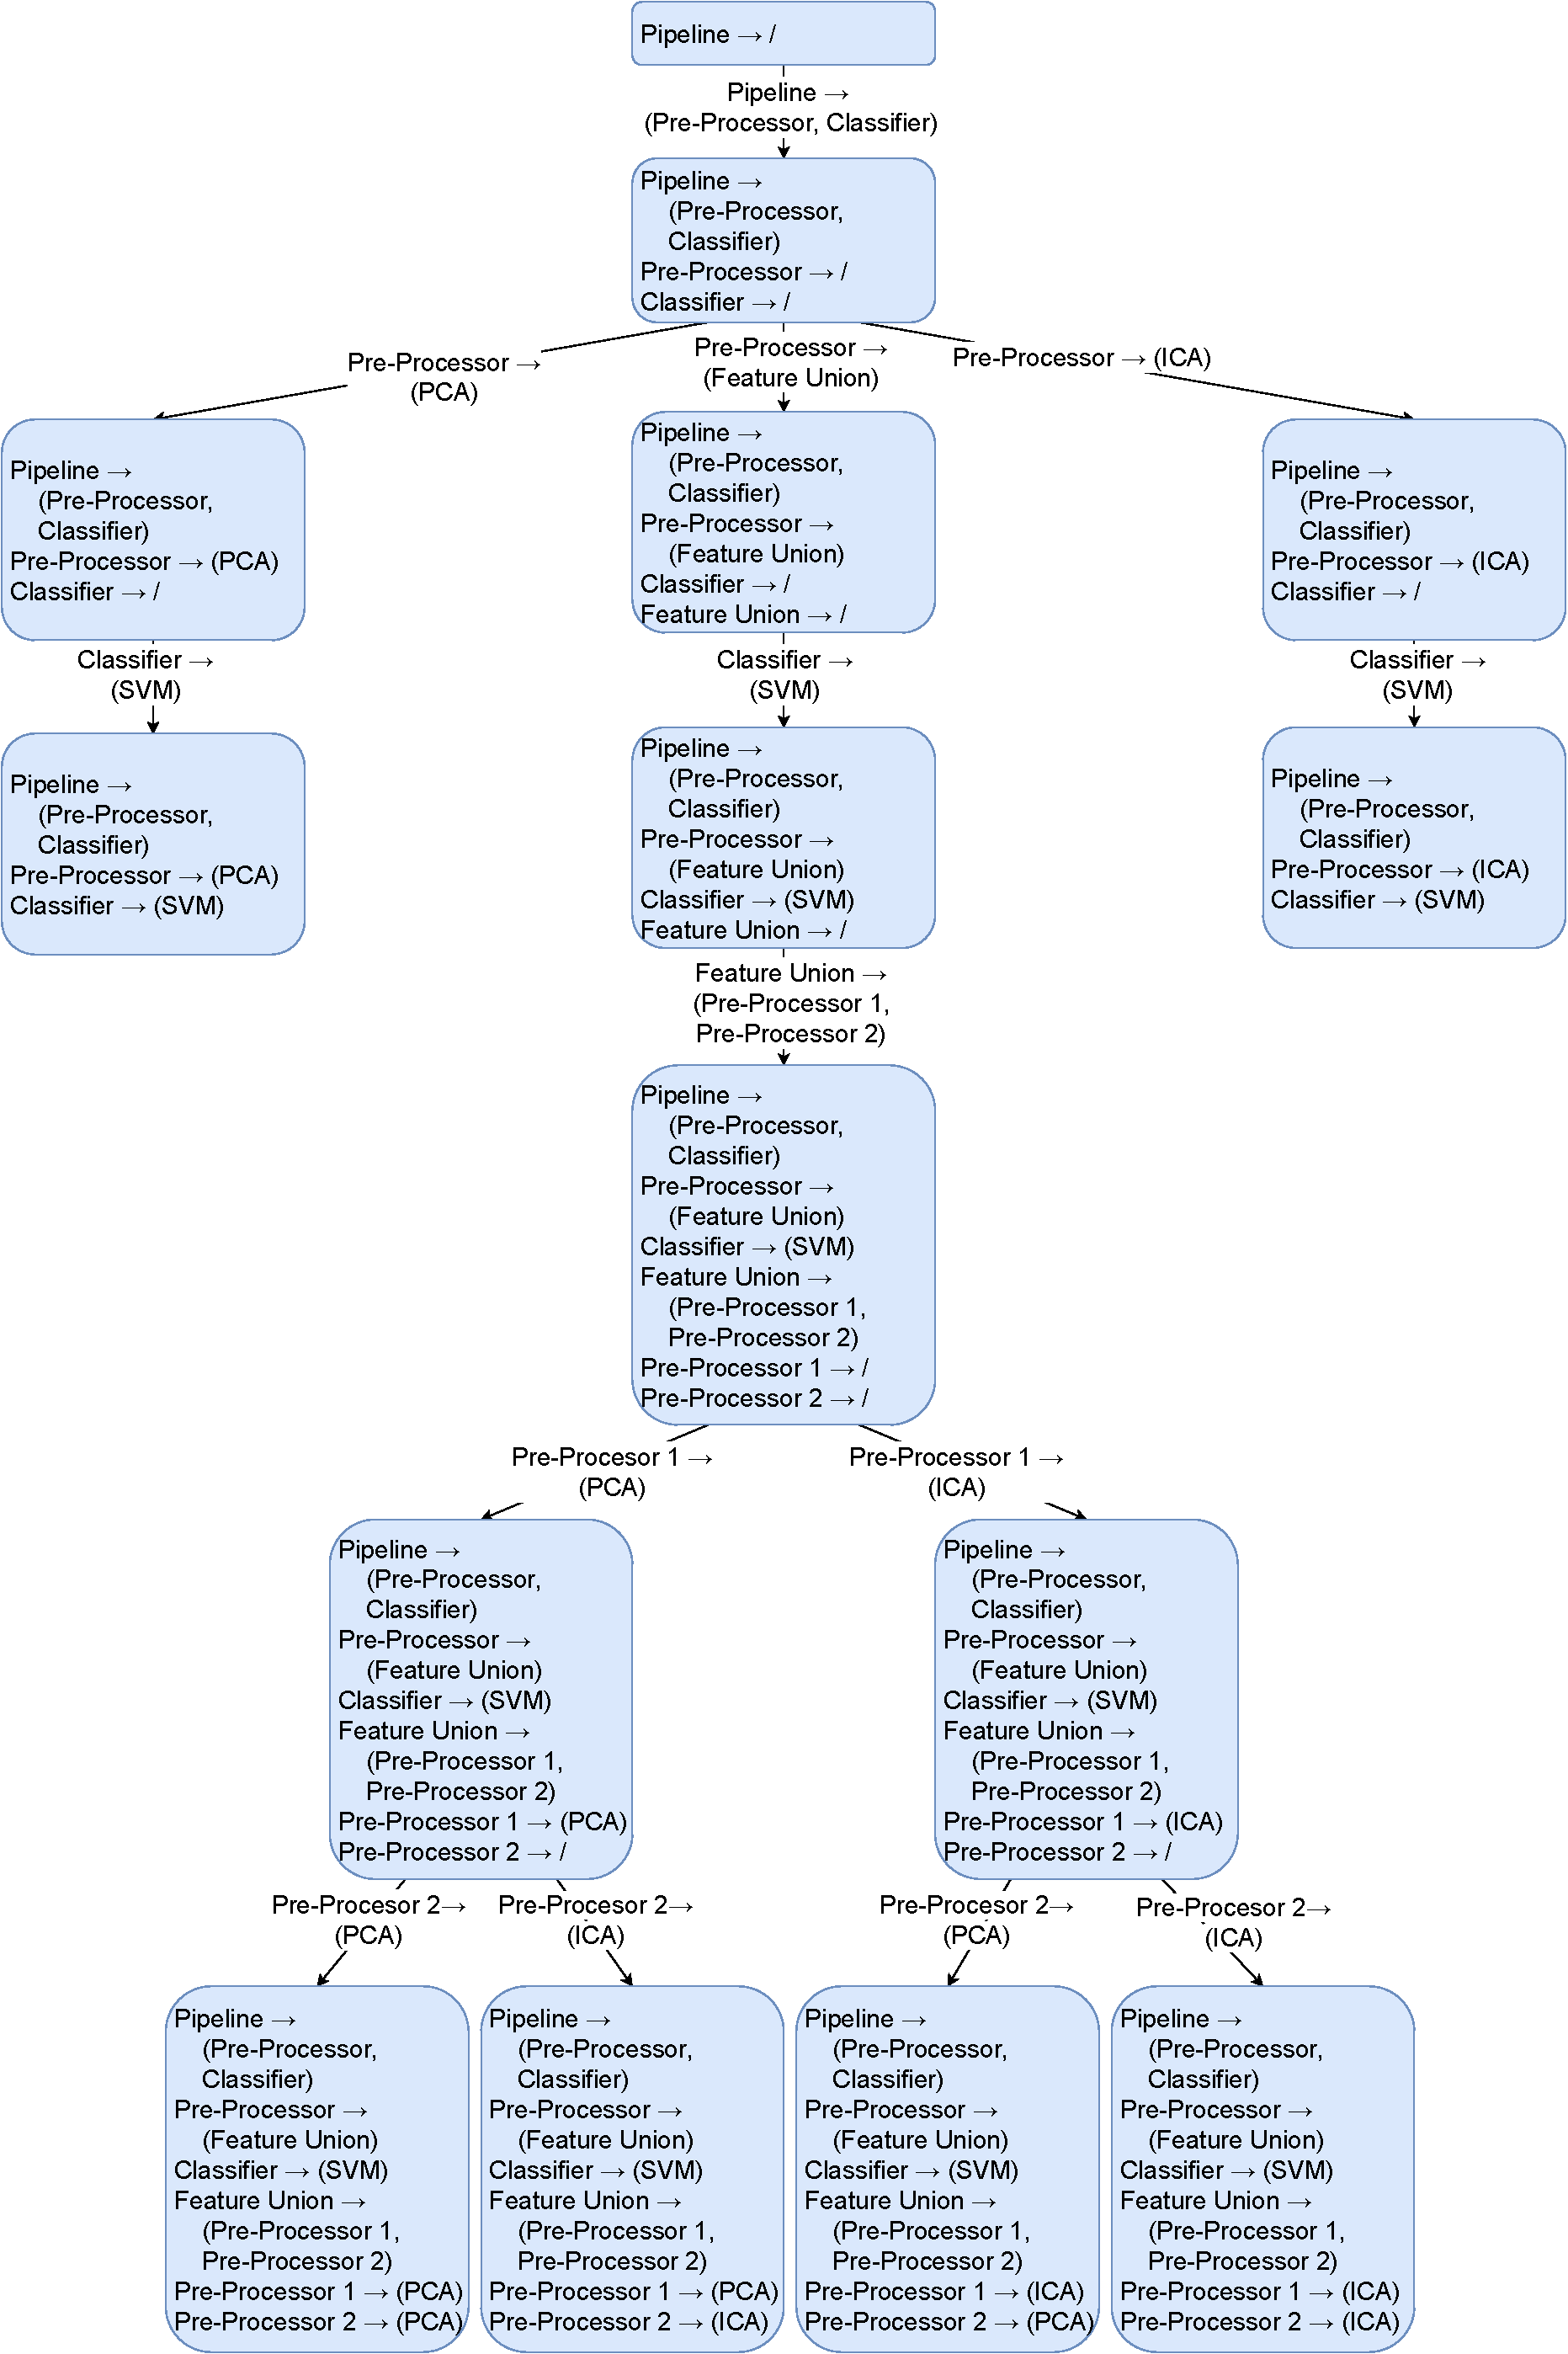
\includegraphics[width=\textwidth]{gfx/Figures/Approach/HTNAutoML.pdf}
    \caption[A complete search graph of an AutoML problem visualized in the HTN context.]{A complete search graph of an AutoML problem visualized in the HTN context. The primitive tasks of this problem are \textit{PCA}, \textit{ICA} and \textit{SVN}.
    All available compound tasks are \textit{Pipeline}, \textit{Pre-Processor}, \textit{Classifier}, \textit{Feature Union}, \textit{Pre-Processor 1} and \textit{Pre-Processor 2}.}
    \label{fig:approach:htn-automl}
\end{figure}

\subsection{Multiple Optimization Algorithms as a Multi-Armed Bandit Problem}
\label{sec:approach:selection:bandit}
All nodes, where every compound task is solved, are therefore leaf nodes and all of them together will be grouped in $N^*$.
Each $n^* \in N^*$ represents a completely defined pipeline $p_{n^*} \in P$ with the internal task-tree of $n^*$, where $P$ is the set of all possible pipelines.
For this $p_{n^*}$, the parameters each included component requires can be aggregated and therewith a model configuration optimization space of the parametrization of $p_{n^*}$ can be deduced.\newline
The approach of this thesis requires a set of optimization algorithms, or alternatively differently configured variants of one optimization algorithm, as an input.
This forms the optimizer algorithms set  $A = \{ a_1, ..., a_k \}$.
To enable the actual model configuration with one of the available optimization algorithms, one additional node for each $a_i \in A$ will be attached as a child node to each model selection leaf node $n^*_j \in N^*$.
The node that is attached to $n^*_j$ as the child node for optimization algorithm $a_i$ is written with the notation $n_{n^*_j}^{a_i}$.
All of these additional nodes for optimization that are child nodes of the model selection leaf nodes $N^*$ are in the node set $N^A = {n^{a_1}_{n^*_1}, ... , n^{a_k}_{n^*_l}}$.
A node with an optimization algorithm $n^{a_i}_{n^*_j} \in N^A$ represents the node that is attached as a child to the model selection leaf node $n^*_j$ and uses the optimization algorithm $a_i$ to optimize a configuration for pipeline $p_{n^*_j}$.\newline
Therefore, the search tree $G=(V, E)$ of the model selection HTN planning is extended for $N^A$ in the form of:
\begin{itemize}
    \item $V'=V \cup N^A$
    \item $E'=E \cup \left( \bigcup_{n^*_i \in N^*} \bigcup_{a_j \in A} n^{a_j}_{n^*_i} \right)$
    \item $G' = (V', E')$
\end{itemize}
Since the nodes in $N^*$ are now not longer leaf nodes of $G'$ they are now referred to as \textit{Pipeline Nodes} and the newly added leaf nodes $N^A$ are the \textit{Optimizer Nodes.}
A simplified illustration of a possible $G'$ without the HTN planning aspects of this extended search tree can be seen in Fig.~\ref{fig:approach:search-graph}.
The pipeline nodes and the optimizer nodes are also marked for a better intuition of the extended search tree $G'$.
\begin{figure}[ht!]
    \centering
    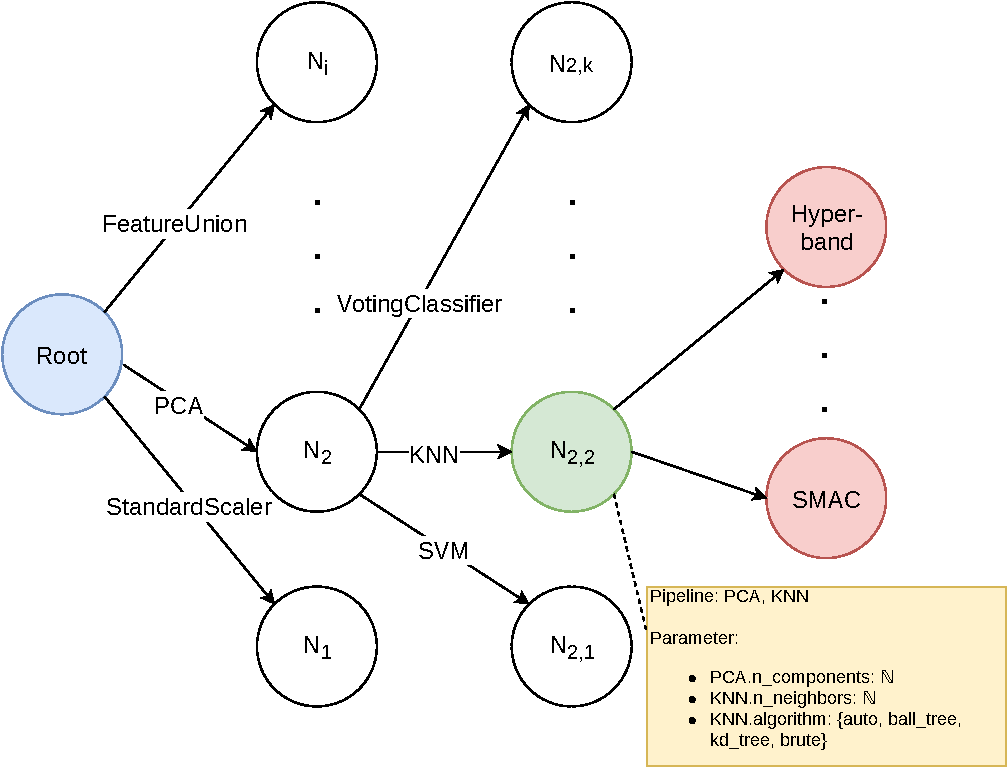
\includegraphics[width=\textwidth]{gfx/Figures/Approach/SearchGraph.pdf}
    \caption[A simplified illustration of a possible extended search tree $G'$.]{A simplified illustration of a possible extended search tree $G'$. The root is drawn in blue, the inner nodes with unsolved task-trees in white, pipelines nodes in green and optimizer nodes in red.
    The yellow box shows the configuration space of the pipeline that is represented by the task tree in that pipeline node.}
    \label{fig:approach:search-graph}
\end{figure}

Now, if a pipeline node is reached, the task arises to select one of the connected optimizer nodes.
The set of optimizer nodes below a pipeline node $n^*_j$ forms the set $N^A_{n^*_j} = \bigcup_{a_i \in A} n^{a_i}_{n^*_j}$.
But without prior knowledge it is impossible to reliably predict, which optimizer is ideally suited to optimize the configuration for the pipeline $p_{n^*_j}$, i.e. to select one node out of $N^A_{n^*_j}$ during a graph search.\newline
A na\"ive approach is to randomly try out different optimization algorithms for optimizing the parametrization and examine their optimization results to gather knowledge successively.
This try-and-error approach is also referred to as \textit{exploration}.
During the collection of exploration results it will become more evident, which optimizer yields which score quality.

Collecting a few sample scores for each optimizer is basically conducting an experiment since black box optimization is often a probabilistic process.
Based on the amount of experiment samples, the optimization capability of an optimizer can be estimated with a certain probability.
After a sufficient amount of samples is gathered, the most suitable optimizer can be selected and utilized with high certainty.
Deliberately selecting and utilizing one specific choice with the expectation of a good result instead of more or less randomly exploring is also named \textit{exploitation}.

The balance between both, exploration and exploitation, is a difficult challenge because of the limited optimization budget.
With too much exploitation it can not be assured with a high probability that the exploited choice is the actual best one, since there is a lack of optimization score samples.
But with too much exploration it may be possible to determine the probably best choice, but there is not enough budget left to actually utilize this choice to a higher extend.
This balance between exploring and exploiting a set of choices, which have an unknown quality, is the fundamental problem of the so called \textit{Multi-Armed Bandit} problems.

A Multi-Armed Bandit problem is usually considered in the context of time steps $t_1, t_2, .., T$, which are sometimes also called turns.
$T$ is in this notation the current turn of the ongoing series, i.e. the current point in time.
For every turn up to $T$, one arm, i.e. one of the $K$ choices $C = \langle c_1, ..., c_K \rangle$, is selected by a selection strategy $s: t \rightarrow [1,K]$.\newline
For a turn $t$, a random reward $r$ is received after selecting the choice $c_{s(t)}$.
Each arm $c_i$ has an underlying probability distribution $D_{c_i}$ for the reward values, i.e. $r_{c_{s(t)}} \sim D_{c_{s(t)}}$.
In the AutoML context, where each arm is one optimizer, this reward could be the testing accuracy score of a pipeline, which is configured with the best found parametrization of the chosen optimizer after a certain optimization budget.\newline
Of course, each distribution $D_{c_i}$ has a corresponding expected value $\mu_{c_i}$.
Therefore, if for example the selection strategy is $s(t) = 1$ the accumulated expected reward is $\sum_{t=1}^T = \mu_{c_1}$.\newline
An optimal strategy $s^*$ would always pick the choice with the highest expected reward $\mu^* = \underset{i \in [1,K]}{\mathrm{max}} \> \mu_{c_i}$, such that $s^*(t) =\underset{i \in [1,K]}{\mathrm{argmax}} \> \mu_{c_i}$.
However, $s^*$ is unknown and has to be approximated by adjusting the constructed $s$ over time.\newline
For every turn where $s(t) \neq s^*(t)$, the strategy looses $\mu^* - \mu_{c_{s(t)}}$ in expected reward.
The exploration vs. exploitation balance problem is here noticeable, since the strategy has to find out the arm with $\mu^*$ by trying out every arm, but also wants to keep $\mu^* - \mu_{c_{s(t)}}$ as minimal as possible via exploitation of an optimal arm.
Otherwise, the difference to $\mu^*$ is expected to grow with every turn where a non-optimal arm is selected.
This idea of keeping the expected reward loss minimal in the overall context of $\underset{T \rightarrow \infty}{\lim}$, such that the strategy has time to approximate $s^*$, is formulated in the form of the \textit{total expected regret}: $R_T = T \cdot \mu^* - \sum_{t=1}^{T} \mu_{c_{s(t)}}$.
Different algorithms for creating such selection strategies $s$ over time can be compared by their respective expected total regret $R_T$, which should be as low as possible.

Selecting an optimizer node out of $N^A_{n^*_j}$ to perform the model configuration of the pipeline $p_{n^*_j}$ can be formalized as a Multi-Armed Bandit problem.
With a given timeout for each optimization run, the optimizers are called repeatedly, which would be the turns of the bandit problem.
The selection strategy for an optimal $p_{n^*_j}$ as well as the most suitable optimizer for a model configuration of this pipeline is unknown beforehand and has to be explored.
But since the time budget is limited, the expected regret of not exploiting this most suitable optimizer for the optimal pipeline is supposed to be as low as possible.\newline
With that assumption of formalizing this selection as a Multi-Armed Bandit problem, there are several existing algorithms to construct selection strategies for optimization nodes until the optimization budget is spent, which balance exploration and exploitation with the goal of keeping the total expected regret minimal.
Common choices are for example \textit{Thompson Sampling}~\cite{Thompson-Sampling} or the usage of \textit{Upper confidence bounds} (UCB) as for instance in the \textit{UCB1} algorithm~\cite{Auer-UCB1}.

\subsection{Ensemble Interaction with MCTS}
\label{sec:approach:selection:mcts}
Let $n^*_j$ and therewith $p_{n^*_j}$ be already selected out of the model selection graph, now there is one arm for each optimization algorithm, i.e. $|A|$ arms.
With this very limited set of arms, any of the referenced Multi-Armed Bandit selection strategy construction algorithms could be applied and with a large enough optimization budget, there is a high probability that the most suitable optimizer will be exploited enough to get a good parametrization for $p_{n^*_j}$.\newline
But since $n^*_j$ is not selected yet because no actual model selection is done until now, there is no pipeline $p_{n^*_j}$ selected and therefore the set of arms cannot be limited to $N^A_{n^*_j}$.
Instead, the set of arms would be the set of optimizer nodes $N^A$, i.e. the set of combinations of all possible pipelines with all optimization algorithms.
This set of combination can be enormously big or even have an infinite amount of elements, depending on the specification of the model selection space.
For such a high number of arms, any Multi-Armed Bandit algorithm would need a massive amount of steps for exploring every arm sufficiently, until an educated guess for a good exploitation candidate could take place.
As a more effective alternative for this use-case, the tree structure of $G'$ should be utilized for a better selection mechanism.

The selection of an optimizer from $A$ for optimizing the configuration of a pipeline $p_{n^*_j}$ is formalized as a Multi-Armed Bandit problem in the form of choosing one of the optimizer nodes $N^A_{n^*_j}$ each turn.
An appropriate Multi-Armed Bandit algorithm will exploit with a high probability the most suitable one of this optimizers $a \in A$ for the specific configuration optimization space of this particular pipeline.
This suitability of an optimizer for a space is dependent on the structure of the space, i.e. the number of dimensions as well as the value sets of the different dimensions, and the properties and landscape of the target function in this space.\newline
Although $a$ is the best optimizer for the configuration space of this specific pipeline $p_{n^*_j}$, this does not apply to all pipelines.
Another optimizer $a'$ could, for instance, be the best optimizer for any pipeline that includes one specific component, which is not part of $p_{n^*_j}$.
In that case, all subtrees below nodes where this component was selected would ideally exploit $a'$ instead of $a$ as the optimization algorithm.
Because such hierarchical dependencies influence the best optimizer choice, the exploration and exploitation of a Multi-Armed Bandit algorithm should utilize this hierarchical dependencies as well.

A \textit{Monte-Carlo tree search} (MCTS) is a heuristic search algorithm, where the heuristic for scoring nodes is based on Monte-Carlo simulations.
With the results of the simulations, an MCTS implementation now needs a selection strategy for the next node that will be expanded.
The aforementioned upper confidence bounds were successively applied as such a selection strategy in the form of the \textit{UCB applied to trees} algorithm (UCT)~\cite{Kocsis-UCT}.
For UCT is the goal to utilize the possibly hierarchical dependencies inside the trees.
Although MCTS does not necessarily has to use this selection strategy, the two terms UCT and MCTS are often used interchangeably.\newline
For UCT and therefore also MCTS, each node has an attached score, which is the basis for selection strategies.
This value can for example be calculated via $\underset{n_i}{\textrm{argmax}} \left( w_{n_i} + f \cdot \sqrt{\frac{\textrm{ln}(t)}{v_{n_i}}} \right)$, but this formula can be adjusted depending on the desired exploration/exploitation behavior.
$w_{n_i}$ is the overall sampled score so far of the subtree below node $n_i$ as an average, $f$ is a factor for the tendency towards exploration, $v_{n_i}$ is the amount of times the subtree below $n_i$ was sampled, and $t$ is the amount of overall turns/iterations so far.\newline
MCTS is usually defined as an algorithm with an iteration of four steps, which are listed in the following and additionally illustrated in Fig.~\ref{fig:approach:mcts}:
\begin{enumerate}
    \item \textbf{Selection}: The next node for expansion is chosen.
    Commonly, each node has a value assigned and starting at the root node, the next node is the child node with the highest value until a not expanded node is reached.
    \item \textbf{Expansion}: The node is expanded, i.e. each possible follow-up state of the state in the unexpanded node is constructed and a child node is attached for each.
    \item \textbf{Simulation}: The new child nodes need some initial scores.
    Since an inner node represent an incomplete state, they are hard to score directly and a heuristic scoring for the subtree below this inner node is necessary.
    A pre-defined number of Monte-Carlo Simulations, which are basically random walks down the search tree until a leaf node is reached, are performed.
    The scores of the states in the found leaf nodes are used to approximate a score for this subtree.
    Thus, the scoring gets more accurate with a higher number of simulations per child node, since more different leaf nodes are reached and therefore more possible solution states are covered.
    But with a higher number of simulations, a bigger portion of the budget is spent each iteration and fewer iterations can be performed overall.
    A careful trade-off is therefore necessary.
    \item \textbf{Backpropagation}: For the child node $n$, the simulations returned some scores $x_1, ..., x_k$.
    Based on this scores, $n$ will receive an initial value.
    Afterwards, every node in the path from the root to $n$ will be updated to incorporate the newly gathered knowledge as well via backpropagation starting at $n$.
    At first, $n$ is scored initially with the following formula $\frac{\frac{\sum_{i=1}^k x_i}{k}}{v_t} + f \cdot \sqrt{\frac{\mathrm{ln} (V_t)}{v_t}}$.
    The formula consists of the following parts: $\frac{\sum_{i=1}^k x_i}{k}$ is the average of the simulation results, $f$ is a pre-defined factor for the focus on exploration, $v_t$ is the amount of visits $n$ had after $t$ rounds of the MCTS loop via previous Monte-Carlo simulations before it was expanded in this round or alternatively 1, and $V_t$ is the visit counter $v_t$ of the parent of $n$.
    For the actual backpropagation, starting with the parent of $n$ which is referred to as $n'$ and continuing until the root is reached, each nodes score is updated similar to the initial scoring of $n$.
    At first, the $v_t$ counter of $n'$ is increased.
    Let $w_{t-1}$ be the scoring of $n'$ of the previous round, it will be updated during the backpropagation of this round with a cumulative moving average $w_t=w_{t-1} + \frac{w_c - w_{t-1}}{t}$, where $w_c$ is the already updated node score of the child node that was the previous stop during the backpropagation.
    Now, the new score of $n'$ is $\frac{w_t}{v_t} + f \cdot \sqrt{\frac{\mathrm{ln} (V_t)}{v_t}}$.
\end{enumerate}
\begin{figure}[ht!]
    \centering
    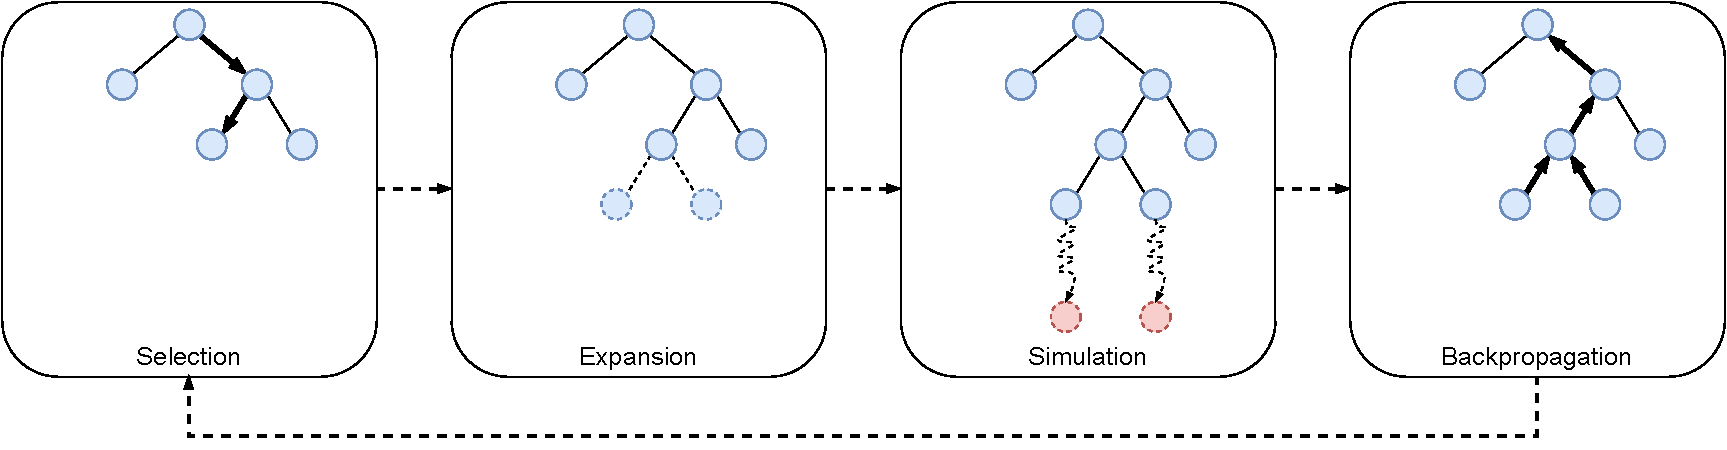
\includegraphics[width=\textwidth]{gfx/Figures/Approach/MCTS.pdf}
    \caption[Illustration of the four MCTS steps.]{Illustration of the four MCTS steps. Inner graph nodes are shown in blue and the leaf nodes that are found during Monte-Carlo simulations are shown in red.}
    \label{fig:approach:mcts}
\end{figure}

To apply MCTS for a model selection in a search tree for example constructed via HTN planning, minor adjustments are necessary.
After incorporating the following changes, this modified MCTS is the algorithmic foundation of the approach of this thesis:
\begin{itemize}
    \item Optimizer nodes are leafs and can not be further expanded. The Monte-Carlo simulations end their search once they find an optimizer node and start an optimization run of the optimizer of this node. If an optimizer node is chosen in the Selection phase, a model configuration run with a given optimization budget is started with the optimization algorithm represented by this node instead of a node expansion.
    \item The main MCTS loop does not run forever or for a fix amount of steps. Instead, it keeps track of the spent optimization budget during the search itself and during the optimizer runs and will stop after the current iteration, if the budget limit is reached or the budget is nearly spent such that it is not possible to perform another complete optimization run.
\end{itemize}
As a user specified configuration, an MCTS model selection implementation with embedded optimizers for model configuration would require some values:
\begin{itemize}
    \item The overall optimization budget $B$.
    \item The budget $b$ a single optimizer run for a Monte-Carlo simulation can spent with $b \ll B$.
    \item The exploration factor $f$.
    \item The number of Monte-Carlo simulations starting at each new child node after expansion.
\end{itemize}
Additionally, the definition of the HTN planning space and the set of optimizers $A$ are required to construct the search tree including the optimizer leafs to achieve an optimizer ensemble for model configuration.
A simplified formulation in high-level pseudo-code of the modified MCTS for the approach of this thesis can be found in Algorithm~\ref{algo:pseudo-code}.
For this simplification are expected as parameters: The overall AutoML timeout, the timeout for each single optimization run, a searchspace created beforehand from searchspace definition files, and the dataset in the format instances $x$ and classes $\hat{y}$.
\begin{algorithm}[H]
    \caption{frankensteins-automl}
    \label{algo:pseudo-code}
    \SetAlgoLined
    \DontPrintSemicolon
    \KwResult{Best found pipeline and corresponding score.}
    \KwData{Timeout, OptimizerTimeout, Searchspace, $x$, $\hat{y}$}
    \BlankLine
    bestPipeline $\leftarrow$ null\;
    bestScore $\leftarrow$ 0\;
    graphGenerator $\leftarrow$ new MCTSGraphGenerator(Searchspace, $x$, $\hat{y}$)\;
    rootNode $\leftarrow$ graphGenerator.getRootNode()\;
    \While{ $\lnot$ Timeout is spent}{
        n $\leftarrow$ rootNode\;
        \While{n is expanded $\wedge \, \lnot$ n is leaf node}{
            n $\leftarrow \underset{c \, \in \, \mathrm{n.getChildNodes()}}{\mathrm{argmax}} $ c.getNodeValue()\;
        }
        \BlankLine
        startNodes $\leftarrow \, \{\}$\;
        \eIf{n is leaf node}{
            startNodes $\leftarrow$ startnodes $\cup$ n\;
        }{
            graphGenerator.expand(n)\;
            startNodes $\leftarrow$ startnodes $\cup$ n.getChildNodes())\;
        }
        \BlankLine
        (reachedLeafNodes, results) $\leftarrow$ monteCarloSimulations(startNodes, OptimizerTimeout)\;
        backpropagate(reachedLeafNodes, results)\;
        \BlankLine
        \For{(pipeline, score) $\in$ results}{
            \If{score $>$ bestScore}{
                bestScore $\leftarrow$ score\;
                bestPipeline $\leftarrow$ pipeline\;
            }
        }
    }
    return (bestPipeline, bestScore)\;
\end{algorithm}

\section{Model Configuration with Multiple Optimizers}
\label{sec:approach:configuration}
With the modified MCTS, the model selection is conducted and additionally it is controlled when an optimizer is started for model configuration.
But since the optimizers of the optimizer nodes $N^A_{n^*_j}$ below the pipeline node $n^*_j$, all try to optimize a configuration for the same pipeline $p_{n^*_j}$, they can utilize the fact they share the same optimization space.
When this sharing and utilization of knowledge about the shared optimization space is achieved, this will be called an \textit{optimizer ensemble} and is in combination with the integration into a search graph the core novelty of the approach of this thesis.\newline
First it is explained in the following, how previous candidate evaluations of the shared optimization space are stored and afterwards, how optimizers re-use this stored candidate scores for new optimization runs, which is often also referred to as warmstarting.

\subsection{Shared Parameter Domain for Selected Models}
\label{sec:approach:configuration:parameter}
In every pipeline node $n^* \in N^*$, the optimization space for the model configuration of pipeline $p_{n^*}$ can be deduced.
Therefore, $n^*$ can be the single point of contact for every subjacent optimizer node $n^{a}_{n^*} \in N^A_{n^*}$.
With this centralized control instance it is possible to store and distribute knowledge from and to the optimizers.

At first, every $n^{a}_{n^*} \in N^A_{n^*}$ can get the concrete model configuration space from $n^*$, as well as other helpful information as for example the default parametrization of certain pipeline components.
Sometimes the default parametrization may be a good starting point, i.e. first evaluation candidate, for some optimization algorithms.\newline
Additionally, each optimizer can store their evaluated candidates together with the evaluation score at $n^*$.
Although this requires additional storage memory, collecting and saving already evaluated candidates has the following advantages:
\begin{itemize}
    \item If saved in a hashtable, candidates can be inserted with a generated key and retrieved with one as well. Therewith, it can be checked if a candidate was already evaluated before and if yes, return the existing score from $n^*$ to the optimizer instead of training and evaluating a pipeline on the dataset again.
    The lookup complexity of a hashtable is constant, while training a machine learning algorithm is generally very time consuming in comparison.
    For example, the complexity of training an SVM with SMO~\cite{Platt-SMO} is between linear and quadratic, depending on the dataset.
    \item If saved in a heap, retrieving the best candidates has a logarithmic complexity and thus, the best $n$ candidates from previous runs of the same or another optimizer from $N^A_{n^*}$ can efficiently be requested from $n^*$ as a starting point for a new optimization run.
\end{itemize}
Memory is in general a comparably cheap hardware component, which can be added to the computer nearly indefinitely such that a lot of evaluation results can be stored.
In comparison, the capacity of the CPU, which affects the time for evaluations, has upper limits.
When these two suitable datastructures are used, the speedup of sharing information about evaluations instead of evaluating once more outweighs therewith the disadvantage of higher memory demands.

\subsection{Warmstarted Versions of Optimization Algorithms}
\label{sec:approach:configuration:warmstart}
If the optimization budget is high enough, there is a high probability that the MCTS will select or the Monte-Carlo simulations will reach a pipeline node more than once.
Meaning that an optimization run is started in a model configuration space where already candidate evaluations have taken place.
Additionally, all these previous candidate evaluations are stored in the pipeline nodes for the given model configuration optimization space.
Hence, the optimization algorithms should utilize this advantage of prior collected data instead of performing the optimization anew from scratch every time.

Starting with a foundation of previously collected data instead of a completely unexplored optimization space is called \textit{warmstarting} an optimizer.
However, it is important to have a certain robustness against local optima, because without it an optimization algorithm could start in a local optimum, which was found in another optimization run, and might not get out of this local optima.
This robustness can be achieved by the optimization algorithms themselves, but additionally a little bit by the selection of the data for the warmstart as well.

In the following it is explained how the optimization algorithms that are used for the optimizer ensembles of this approach can be modified to be executed warmstarted.
All this optimization algorithms are established black box optimization algorithms, which were presented in~\ref{sec:theory:optimization:search} up to~\ref{sec:theory:optimization:bayesian}.
They will therefore utilize an ordered list of pairs of already evaluated candidates in the form of $l = \langle (c_1, s_1), ... (c_k, s_k) \rangle$, where $c_i$ is an already evaluated pipeline configuration and $s_i$ the corresponding score of this evaluation.
The list $l$ is created from a subset with the top $|l|$ candidates out of the set of all previous evaluations and $|l|$ can be decided by the corresponding optimization algorithm.

\subsubsection{Random Search}
The first variant of a random search, where each candidate was drawn independently and at random, has no advantages from warmstarting besides not having to re-evaluate candidates that were already evaluated.\newline
But the second variant of a random search, where a candidate is sampled out of the hypersphere around the current best candidate up until either the optimization budget is spent or no improvement happened for $i$ iterations, can profit from a modification to a warmstarted version.
This version could use the top pair of $l$, or alternatively one randomly chosen pair  out of the top $n$ pairs of $l$ for more variation, as a starting point.\newline
Now, the random search will start sampling candidates in the hypersphere around this starting point and has the chance to find a better neighboring configuration, because it already is in a candidate with some good previous evaluations.\newline
Of course the chosen starting point could be a local optimum, but this random search variant will use this hypersphere for at most $i$ iterations if no improvement is achieved, which can be an indicator for an optimum.
In this case, it will select a new random starting point.
Thus, not more than $i$ iterations are lost to a local optimum selected from $l$, which is depending on the optimization budget usually manageable, since random search is a comparably simplistic and therefore fast optimization algorithm.

\subsubsection{Hyperband}
Hyperband is basically a method of treating multiple, parallel running random searches as a Multi-Armed Bandit problem and stopping the less successful instances to have more optimization budget for the better performing instances.
Therewith, if each random search instance is implemented as the warmstarted version from the previous explanation, Hyperband can profit from warmstarting as well.\newline
The typical Multi-Armed Bandit problem of balancing exploration and exploitation should be applied here as well.
If Hyperband is configured to have $k$ parallel running instances, $\lfloor \sigma \cdot k \rfloor$ instances with $\sigma \in (0,1)$ should start in the direct neighborhood of one of the top candidates from $l$ for exploitation, while $\lceil (1 - \sigma) \cdot k \rceil$ instances should start at new and randomly chosen configurations for a better exploration coverage of each Hyperband run.

\subsubsection{Genetic Optimization}
A very important part of a genetic optimization algorithm, is the selection scheme with which individuals from the last generation will be selected to construct the next generation.
Such a selection can be a na\"ive approach, as for example a random selection or the best individuals from the current generation.
But it can also be a more sophisticated scheme as for example a \textit{Boltzmann Tournament Selection}~\cite{Goldberg-Boltzmann}.\newline
With such a selection scheme in place, the warmstarting can be implemented straightforward.
Instead of selecting individuals with a selection scheme from a previous generation, the selection scheme of the genetic algorithm will be applied on $l$.
Therefore $|l|$ is set to the value that is used as the population size.\newline
Alternatively it is also possible to re-use the Hyperband warmstarting approach, such that $\lfloor \sigma \cdot k \rfloor$ candidate are selected via the selection scheme from $l$ and $\lceil (1 - \sigma) \cdot k \rceil$ candidates are randomly created to achieve more variance and a certain robustness against local optima.

\subsubsection{SMAC}
For the Bayesian optimization implementation \textit{SMAC}, a warmstarted variant was developed by~\textcite{Lindauer-Smac-Warmstart}.
During the optimization, SMAC trains a regression model, for instance a Random Forest, to predict the performance of a configuration before actually evaluating it.
This regression model is then used to guide the selection of candidates that are actually evaluated to build the surrogate function model.
Additionally to training this regression model progressively during the optimization, it can be trained beforehand with $l$ or any other subset of all previously evaluated candidates to have a more accurate regression model right from the start of the optimization run.

\subsubsection{Discretization Search}
This optimization algorithm is based on the optimization method from \textit{ML-Plan}, where the inner nodes of a search tree are used to further discretize one dimension of the optimization space at a time with each node.
This is achieved by refining the ranges of the dimensions, i.e. splitting them, into several value ranges.
For each split a child node is attached during a node expansion until, depending on the parameter type, either the interval only consists of one value or the splits interval size is below a given threshold.
Afterwards the next dimension is refined, until each dimension was completely discretized and a leaf node is reached.\newline
Therefore, this can be viewed as converting a grid search approach into a tree structure, which will be searched more dynamically then a grid search, with a best-first search, where the nodes are scored via Monte-Carlo simulations.\newline 
In ML-Plan the optimization was done for model selection and model configuration in a joint graph.
Here for this approach, instead of creating a search graph for the complete AutoML problem solution space, it is solely applied on the model configuration space, i.e. hyperparameter optimization.\newline
Warmstarting does here not imply that a starting point of the optimization is selected out of $l$, because the selection is controlled by the best first search depending on the node scores.
However, if the same optimizer instance is started more than once, this optimization approach can be warmstarted in the way that a search graph is already created for this space and the search can simply be continued.
